\begin{savequote}[75mm]
``Humans are allergic to change. They love to say, `We've always done it this way.'' I try to fight that. That's why I have a clock on my wall that runs counter-clockwise.''
\qauthor{Grace Hopper}
\end{savequote}

\chapter{Discussion}\label{discussion}
\setcounter{figure}{-1}
\setcounter{table}{-1}
\setcounter{section}{-1}
\setcounter{NAT@ctr}{-1}

\begin{figure}[t!]
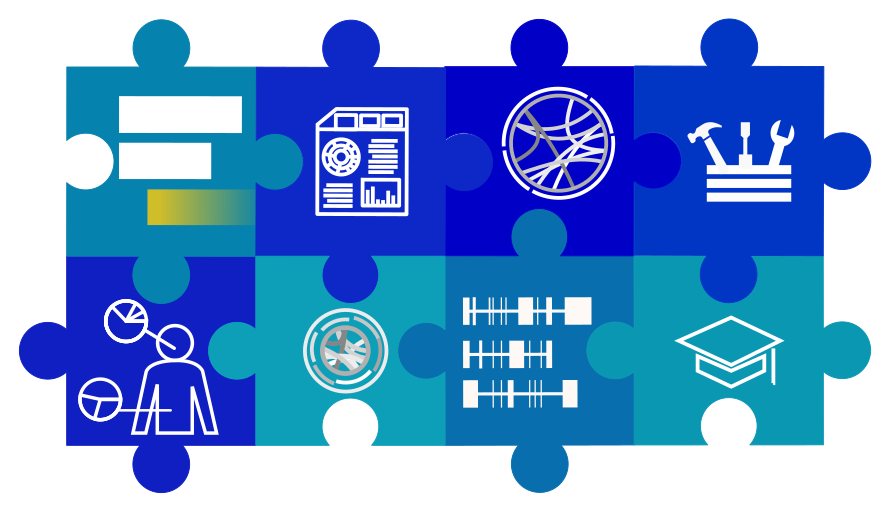
\includegraphics[height=15em]{frontmatter/images/chapter-header-discussion-tools.png}
\end{figure}
\setcounter{figure}{-1}
\setcounter{table}{-1}
\setcounter{section}{-1}

Since the completion of the human reference genome in 2003, the field of molecular biology has been transformed almost beyond recognition, and along with it, the field of bioinformatics has evolved from a niche discipline to an integral part of every biomolecular research question. Where mere decades ago most genomic data analyses could largely be performed by hand, nowadays they often require a supercomputer. Programming knowledge is required to run such analyses, but biomedical scientists are not typically trained in these skills, and have thus become reliant on bioinformaticians to carry out this work for them. Similarly, bioinformaticians often lack the increasingly complex biological knowledge required to fully interpret the results~\cite{preeyanon2014reproducible}. Biologist and bioinformatician must therefore work together closely, and each should be trained in the other discipline in order gain awareness of factors that might influence analysis or result interpretation.

Furthermore, data is being generated at an exponential rate (while bioinformaticians are not), and one way to address this gap is to empower researchers and clinicians to run their own day-to-day analyses without the need to consult a bioinformatician at every step. A way towards delivering this is through the creation of accessible analysis tools and platforms and sufficient training resources.


\section{Galaxy for open and accessible research}
The Galaxy project~\cite{giardine2005galaxy,blankenberg2010galaxy,afgan2016galaxy} --with the latest update paper \cite{afgan2018galaxy} in \hyperref[chapter:galaxy]{Chapter~\ref{chapter:general}}-- is a framework that enables the empowerment of researchers to run complex data analysis without programming expertise. The Galaxy project is free and open-source and has an active user and community. Galaxy encourages feedback and code contributions from its users to improve and evolve along with the ever-changing landscape that is bioinformatics. \hyperref[chapter:galaxy]{\textbf{Chapter~\ref{chapter:general}}} outlines the ongoing development in the Galaxy framework.

The set of tools wrapped into Galaxy by both the user community and the core development team continues to increase exponentially, and the number of tools in the tool shed has now surpassed 7200. New core features are also continually incorporated into the Galaxy code base in order to facilitate the needs of users. For example, scalability is an important area of development, and continual efforts are made to ensure the platform can keep up with the current \emph{big data} explosion. To this end, several improvement were made to assist users with the handling of large datasets, such as the introduction of dataset collections and the rule-based uploader. Dataset collections allow large numbers of files to be analysed with minimal effort, and the rule-based uploader supports the specification of experimental design files at upload time to import and structure large sets of data files. In terms of server scalability, Galaxy supports integration with a multitude of workload managers and compute infrastructures.

Accessibility of the Galaxy platform was improved by the integration of a new help forum, the introduction of interactive tours to faimilarize users with the Galaxy interface, and through the development of a central repository of Galaxy-based training materials (\hyperref[chapter:galaxy]{Chapter~\ref{chapter:training}}). Furthermore, the Galaxy Hub was developed, the one-stop shop for finding all things Galaxy, whether it be events, documentation, training, public Galaxy servers or scientific publications using Galaxy. These efforts to enhance accessibilty of the Galaxy platform appear to be paying off, given the exponentially growing number of scientific publications that refer to Galaxy~\cite{url-zotero-galaxy}.


\section{Training}
Training is an essential component in the dissemination of accessible bioinformatics tools and workflows. The Galaxy platform is especially well-suited for the delivery of bioinformatics training because it provides a layer of abstraction that allows trainees to focus on the bioinformatics \emph{concepts} rather than the implementation details of the tools. Without this separation, trainees would have to simultaneously learn about the UNIX commandline or programming environment, on top of the bioinformatics topics at hand. This would increase the cognitive load and hamper the learning process~\cite{paas2003cognitive}. Given this observation of Galaxy's suitability for use in training, the Galaxy Training Network (GTN)~\cite{url-gtn} was formed; a loosely-defined open group of instructors around the world who use Galaxy for training purposes. Initially there was little coordination between the different instructors in terms of materials used, and thus a lot of duplication of effort. There was a clear need for centralisation of training materials and knowledge sharing within the trainer community. Chapter~\ref{chapter:training} describes the community-driven web-based framework for the delivery of bioinformatics training using the Galaxy platform that we developed in response to this need.
Our aim was to create a fully open and transparent framework that is accessible and easy to use for both trainees and trainers. The materials are centered around \emph{research stories}; usually the recreation of results described in published papers. This gives trainees the confidence that the tools and pipelines are practically useful and of publication-level quality, as well providing them with the opportunity to dive deeper into the science and informatics behind the training. Since the creation of this training platform, a number of scientific publications have included Galaxy training materials as a form of documentation and illustration of the presented analysis pipelines~\cite{gruning2017rna,blank2018disseminating,batut2017asaim,hiltemann2018galaxy}.

One of the main challenges in designing this framework was to allow easy contributions from instructors, without the need for any web development knowledge. To this end, we used Jekyll templating~\cite{url-jekyll}, which allows tutorials to be written in the simple and accessible markup language called Markdown~\cite{url-markdown} which can be rendered as HTML. Analogous to how Galaxy allows scientists to run analyses while being abstracted away from the implementation layer of the tools, this approach allows instructors to create web pages for their tutorials without being concerned with the the syntax and intricacies of the web application layer.

A further challenge was to enable the materials to be usable both by instructors during workshops, and by individuals learning on their own. This is accomplished by including all materials instructors might provide during a workshop in the GTN training materials framework. This includes introduction slides as well as hand-on materials, input datasets and workflows, further reading suggestions, and an automatically updated list of available Galaxy servers which meet the requirements to run a given tutorial. Furthermore, learning assessments are provided in the form of question boxes, answers to which are included within the materials (in an initially hidden state) for trainees to verify their understanding of the materials. If further assistance is required, links to support channels such as a help forum and chat rooms are provided.

The community-driven nature of the training framework is essential for the long-term survival of the project; it allows for the distribution of the maintenance burden and takes advantage of the combined expertise present in the community. All development happens on GitHub~\cite{url-github}, where anybody may suggest additions or changes, and any such proposed changes are thoroughly tested using the Travis continuous integration system~\cite{travis-ci} to ensure functionality and adherence to guidelines. The proposed changes are subsequently reviewed by one or more of the dedicatied topic maintainers, or other volunteers from the community. Once approved, the code is merged into the main code base, and the new website is automatically built and deployed using Travis and GitHub. In order to assess the quality of the tutorials and identify areas of improvement, feedback from both trainees and instructors is indispensable. To this end, we integrated evaluation forms at the end of each tutorial, and hold regular community meetings with training developers and trainers.

As Galaxy evolves, so will the associated tutorials; where Galaxy is expanding beyond bioinformatics and is now also being used in fields such as natural language processing and computational chemistry, so have we noticed a steady expansion of topics and tutorials contributed by the community. In the year following the publication of Chapter \ref{chapter:training} , we saw 6 new topics added, 66 new tutorials, and the number of contributors grew from 64 to 137.

While the focus of development in this project initially lay with improving the experience for end-users of the tutorials, our focus is now shifting to increasing support for tutorial contributors and instructors intending to use our materials. The main challenge in the coming years will be the community management; creating and sustaining a close-knit community of Galaxy users and instructors so that the project can survive even when its original developers have moved on.


\section{Visualisation and Reporting}
Visualisation is an essential component to aid in interpretation of big and multidimensional datasets. Tools such as Circos \cite{circos} allow for the visualisation of multiple large and complex datasets in a single circular plot. Circos is highly customizable, but this high degree of flexibility comes paired with a high degree of complexity and a steep learning curve. To improve the user-friendliness of this tool and improve its interoperability with upstream tools, we developed Galactic Circos (Chapter~\ref{chapter:general}), integrating Circos into Galaxy, and providing a set of preprocessing tools to facilitate interoperability with a wide range of output formats produced by upstream tools.

Galaxy in its current form lacks an appealing system of results summation and reporting. While Galaxy sports a plugin system for visualisation of individual datasets, a generic reporting tool for displaying a set of workflow outputs together does not exist. To this end, we developed iReport (Chapter~\ref{chapter:general}); a fully customizable Galaxy tool for the generation HTML reports capable of displaying any number of workflow outputs.
iReport is intended to be used as the final step of a workflow; in this manner, end-users need only to open a single workflow output to get a full overview of results. The developer of the workflow can fully tailor an iReport to the needs of their end users (e.g. clinicians), including the ability to add links to datasets and external resources, create searchable and sortable tables, embed images and custom text, and to divide content into different pages.
By adding such a summarizing report at the end of an analysis pipeline, clinicians and other end users are able to run workflows and view results with minimal instruction or knowledge of the Galaxy interface.

Galaxy is a highly flexible analysis platform, which is very useful for researchers still developing their pipelines, but for clinicians who have fixed and validated workflows, the flexibility is no longer required, and in many cases even undesirable. By utilizing the Galaxy API, simplified web front-ends for Galaxy may be created (e.g. Galaksio~\cite{klingstrom2017galaksio} and IRIDA~\cite{matthews2018integrated}), such that only those features needed by the users are exposed in the user interface. In the case of clinical applications, this provides the additional benefit of minimizing the chances of incorrect invocations of the validated workflows by the end user.

\section{Use Cases}

The concepts and tools described in the previous sections were applied to two separate use cases. Chapters~\ref{chapter:fusiongenes} and~\ref{chapter:virtualnormal} describe the creation of analysis tools and pipelines for variant analysis in prostate cancer research. In Chapter~\ref{chapter:microbiota}, Galaxy-based analysis pipelines were developed and tested for the application of NGS-based microbiota profiling for clinical diagnostics.


\subsection{Cancer Analysis: Fusion Gene Detection}
\subsubsection{The Bio}

Prostate cancer is one of the most commonly diagnosed cancer types in men, and while many patients present with an indolent form of the disease, others develop a highly aggressive tumour type, and overall, prostate cancer is among the top 10 leading causes of cancer-related deaths in men~\cite{jemal2010global}. Cancer is a disease of the genome, where accumulation of mutations over time drive the progression of the illness. Genome sequencing approaches can be used to extensively explore these genomic alterations in cancer, including small variants and larger structural variants (SVs), within or ouside genes.

While mutations that affect the protein-coding regions of the genome have been widely studied, the impact of non-coding mutations and structural variants in cancer remain largely undefined~\cite{cuykendall2017non,khurana2016role}. The advent of whole-genome sequencing techniques has enable the characterization of SVs and other mutations not detectable by exome-based approaches. Fusion genes may arise when structural variants (SVs) occur within two different genes, causing the creation of hybrid genes with the potential to produce hybrid proteins that may disrupt vital cell functions.  For example, the presence of the \emph{TMPRSS2-ERG} gene fusion is observed in approximately 50\% of prostate cancer patients and many other less frequent fusions have also been identified~\cite{tomlins2005recurrent}. Detection of fusion genes may aid in the diagnosis or treatment of cancer~\cite{nowell1960chromosome,nowell1961chromosome,druker2001activity,druker2001efficacy}.

Chromothripsis is a phenomenon observed primarily in cancer cells, that involves the shattering and subsequent imprecise repair of one or more chromosomes in a single catastrophic event. Chromothripsis is characterized by the observation of 1) large numbers of chromosomal rearrangements on a localized parts of the genome, 2) alternations between a small number of different copy number states, and 3) alternation between regions displaying a loss of heterozygosity (LOH) and those with preserved heterozygosity~\cite{maher2012chromothripsis}.

Chapter \ref{chapter:fusiongenes} describes the identification of chromothripsis in the 5q arm of the VCaP cell line. A very large number of SVs were detected, and copy number varied primarily between two copy number states states, with only sporadic occurrences of a third state. This alternation between a small number of copy number states suggest the rearrangements were precipitated by a single catastrophic event.

The 573 rearrangements involving this part of chromosome 5 were then investigated for their potential to lead to the formation of fusion genes using the iFUSE application also presented in Chapter \ref{chapter:fusiongenes}. Out of this large number of rearrangements, only 18 were found to occur between two different genes at a consistent orientation. These fusion gene candidates were confirmed via sequencing using custom PCR. This allowed 16 out of 18 fusion candidates to be confirmed on the DNA level, although only 5 of these were also measured on the mRNA level, suggesting instability of the fusion transcripts or down-regulation of the expression of these fusion genes.

Overall, this research has shown that any studies involving this commonly used prostate cancer cell line should take the presence of chromothripsis on chromosome 5q into account. Furhtermore, this study highlights the potential utility of this cell line as a model for research on chromothripsis.

\subsubsection{The Informatics}
Whole-genome sequence experiments typically generate very large output files. Furthermore, in the case of structural variant analysis, the output file formats lack consistency across tools and sequencing platforms, and interpretation is greatly aided by visualisation and annotation with external data resources. To this end, the iFUSE application was developed, creating a visual representation of fusion gene candidates and computing various metrics such as predictions of fusion protein product.

While iFUSE provides valuable aid in interpretation on a per-event basis through its visualisation and annotation, it is less suitable for obtaining a genome-wide overview of structural rearrangements. Large-scale rearrangements such as chromothripsis for instance are easy to miss when examining the raw textual output files or the iFUSE visualisations. In order to evaluate the presence of chromothripsis, a more high-level view of the genome is needed, and to that end, whole-genome visualisations were created using Circos~\cite{circos} for rearrangements, and GNUplot~\cite{url-gnuplot} for the copy number and heterozygosity plots. This approach enabled the instant identification of chromothripsis present in the VCaP sample, which could then be followed up by closer examination of individual rearrangements involving the chromosome 5q using iFUSE.

Both the iFUSE application, the Circos Galaxy wrappers, and the other tools and visualisations created in this chapter are open-source and publicly available on an example server, and are accompanied by extensive documentation to enable re-use by institutes that may have legal restrictions about the use of clinical samples on public servers.

\subsection{Cancer Analysis: Somatic Mutation Determination}
\subsubsection{The Bio}
One of the main challenges in analysis of oncological samples is the identification of those mutations that potentially function as oncogenic drivers, and the large number of passenger mutations or polymorphisms present in the germline of the patient that are typically deemed to be functionally benign~\cite{lawrence2013mutational}. To this end, a sample of normal tissue from the same individual is often sequenced in conjunction with the tumour sample. This allows the subtraction of germline variants from the set of mutations detected in the cancer sample, in order to narrow down the set of potential driver mutations. However, in practice such an associated normal sample may not always be available, for a variety of reasons. In such cases, an alternative approach is required.

Given the observation that the majority of any individuals germline variants are polymorphic and observed frequently throughout the human population~\cite{10002010map,10002012integrated}, in combination with the exponential increase in publicly available genomic datasets, we explored the feasibility of constructing a so-called \emph{virtual normal}, consisting of a reference set of variants found in the population. Chapter \ref{chapter:virtual-normal} describes this investigation.

Our approach used a set of over 900 publicly available whole genomes from healthy, ethnically diverse individuals. We combined this with the customary approach of annotating variants for presences in several online databases of polymorphism in the human population. We tested the performance of our method using 4 different tumour samples with associated normal samples, 2 of which had been sequenced on two different platforms (Complete Genomics and Illumina).

Our results show that while highly unique personal variants cannot be 100\% corrected for, a significant number of variants observed in the tumour sample also occur in the virtual normal set of genomes, and thus can be corrected without the need of an associated normal sample from the same individual. As more and more WGS samples are made publicly available, increasingly rare variants may be corrected for in this manner. Furthermore, we demonstrated that the use of a virtual normal provided a significant improvement over relying solely on annotation with online variant databases. This observation seems counter-intuitive given that these databases often contain variants originating from tens of thousands of sequencing experiments; far more genomes than the virtual normal. However, this result can be explained by noting that the virtual normal approach preserves the genomic context of variants (e.g. adjacent variants in the same sample), while this contextual information is lost when variants are submitted to variant databases. To understand why this contextual information is so important, one must realize that many mutations can be described in multiple different yet equivalent ways, and the only way to resolve this equivalency is to take the genomic neighbourhood of the variants into account. This enables more advanced comparison algorithms to resolve equivalency of variants where routine position-based exact comparison method fall short.

A combination of all 3 correction methods (matched normal, virtual normal, and variant databases) yields optimal results, but when faced with a choice between a virtual normal or a matched normal, both approaches performed roughly equally well. Without an associated normal, personal germline variants may be erroneously deemed somatic, but conversely, omission of the virtual normal led to a roughly equal number of false-positive somatic variants. This can be explained by a combination of sequencing errors or suboptimal variant calls in the associated normal sample, and the general difficulty present in variant comparison analyses.

Depending on the use case, the decrease in power to detect highly personal germline variants may be offset by the decrease in cost from the absence of the necessity of sequencing a matched normal sample with every tumour sample.

\subsubsection{The Informatics}
The samples in this study were sequenced by Complete Genomics~\cite{drmanac}, a sequencing service which delivers both raw sequencing data and post-processed results. Complete Genomics provide a suite of commandline tools for handling and downstream analysis of their often custom file formats. As a first step towards building the virtual normal analysis pipelines, these existing tools were wrapped into Galaxy. On top of these third party tools, several custom analysis components had to be created, as well as several file format conversion steps to function as a \emph{glue} between steps. The full suite of analysis tools has been made publicly available on GitHub, as well as detailed instructions on where to obtain the virtual normal genome set, and how this may be extended with additional normal samples in the future.


\subsection{Microbiota Profiling for Clinical Diagnostics}
\subsubsection{The Bio}
The MYcrobiota project described in Chapter~\ref{chapter:microbiota} was aimed at developing a 16S microbiota profiling pipeline suitable for use in clinical diagnostics. While 16S rRNA sequencing is a relatively well-established technique, there are several obstacles to overcome to enable its use in routine diagnostics. These obstacles include 1) the high prevalence of chimera formation during PCR amplification~\cite{huttenhower2012structure}, 2) the inability to standardize the relative abundance results obtained from 16S profiling across different studies, and 3) the lack of a user-friendly bioinformatics pipeline that can be operated by clinicians without extensive bioinformatics knowledge.

The MYcrobiota platform is the result of a close collaboration with Streeklab Haarlem~\cite{url-streeklab}, a microbial diagnostics lab servicing a large number of GPs and hospitals in the region. In order to facilitate the use of 16S rRNA sequencing in a diagnostic setting, several enhancements to standard procedure were required, both in the wet lab and the bioinformatics pipelines to overcome the aforementioned obstacles.

The MYcrobiota platform utilizes the micelle PCR (micPCR) method~\cite{boers2015micelle,boers2017novel}. In this approach, PCR amplifications of each template 16S template sequence occurs in a physically distinct reaction environment called a micelle, thus greatly reducing the generation of hybrid sequences known as chimeras. This approach has the additional benefit of allowing for the absolute quantification of abundance by eliminating PCR competition induced bias. To further improve the accuracy of the results, each sample was sequenced in triplicate and averaged in order to eliminate any remaining quantification bias in the micPCR protocol. A further correction was performed using a negative extraction control sample that was sequenced with every batch. Finally, and internal calibrator (IC) was used to enable quantification of each resulting OTU in terms of the number of gene copies rather than relative abundances. This IC consisted of a known quantity of a bacterium not present in the natural microbial flora under investigation, and was added to the samples before PCR amplification.

Results were validated through the analysis of 47 clinical samples obtained from patients presenting with a variety of damaged skin conditions, and results were compared to the culture-based methods currently employed for routine clinical microbial diagnostics. The results showed that the vast majority (>95\%) of genera detected by routine culturing were also detected by the MYcrobiota platform. Conversely, the majority of bacterial taxa detected by MYcrobiota were not identified by culture. Many of these additional genera detected were anaerobes consistent with previous studies \cite{price2009community}, and included potential pathogens such as \emph{Kingella} not detected in routine culture.

The universality of the MYcrobiota pipeline has been subsequently demonstrated through its application to environmental studies in drinking water distribution systems~\cite{boers2018monitoring} and in a clinical setting involving patients presenting with suspected septic arthritis~\cite{boers2018detection}.

It must be noted however, that certain limitations to the MYcrobiota remain, and further development and extensive clinical validation studies are required before introduction into routine diagnostics. For example, the current methodologies lack the discriminative power to differentiate to the species taxonomic level, which is often essential for clinical diagnostics. However, results could be supplemented with species-specific PCRs. Alternatively, relatively simple alterations to the current MYcrobiota platform could accommodate approaches such as the sequencing of multiple hypervariable regions or full-gene 16S rRNA, as well as other potential genetic markers such as \emph{rpoB}~\cite{adekambi2009rpob}, \emph{gyrB}~\cite{yamamoto1995pcr}, the ITS region~\cite{schoch2012nuclear}, or one of many other potential markers capable of differentiation of prokaryotes at the species taxonomic level \cite{lan2016marker,sabat2017targeted}.

In conclusion, the development of the MYcrobiota platform paves the way for the introduction of culture-free quantitative microbiota profiling methods into clinical diagnostic laboratories. It is capable of providing a highly accurate and comprehensive profile of the microbial composition of clinical samples, even at low biomass, and may provide clinicians with valuable information on potential pathogens not (easily) provided by the standard culture-based methods. Alternatively, the culture-negative status of clinical samples may be confirmed by the absence of 16S rRNA gene copies in the MYcrobiota results.

\subsubsection{The Informatics}

\textbf{Tools}. As a first step to creating the MYcrobiota platform, we incorporated the full suite of 125+ mothur tools~\cite{schloss} into Galaxy, as well as the Krona~\cite{ondov2015krona} tool, and Phinch~\cite{bik2014phinch} display application for visualisation of tools. To facilitate the interoperability of these tools and others already available in Galaxy, we also created some file format conversion tools to function as the \emph{glue} between steps and facilitate the interoperability with existing downstream tools through the support of widely used file formats such as the BIOM format~\cite{mcdonald2012biological}.


\textbf{Workflows}. In order to optimize utility of the tools, several standard pipelines were provided in Galaxy, based on available standard operating procedures (SOPs) defined in the research community. However, for use as clinical pipelines, further customizations were required, for instance to support the experimental setups utilizing such methods as replicates, negative extraction controls, as well as additional alterations necessitated by the use of micPCR protocol such as the use of an IC for quantification. To accommodate these custom requirements, the standard pipelines had to be augmented with additional components and custom parameter settings, arrived at through a lengthy cycle of testing and adjustment, followed by clinical validation. In order to facilitate scaling of these analysis, the pipelines utilize Galaxy collections, enabling analysis sizes from single samples to tens of thousands of samples.

Because this workfloow was intended for use directly in the clinic, extensive validation of the tools and workflows was performed, in collaboration with the Streeklab Haarlem. This included testing of the individual workflow components (tools), as well as the entire end-to-end analysis pipeline. Testing was performed using public datasets, artificially constructed samples, and previously analyzed patient samples. By analyzing mock communities, we were able to test the entire experimental pipeline, from sequencing to bioinformatics, and create and estimation of the error rates. In the final report at the end of the workflow, a set of QC metrics is presented to the user, to aid in the quick identification of potential problems with the sequencing or subsequent analysis, by flagging metrics outside the range of expected values based on the validation process.

\textbf{Visualisation and Reporting}. The MYcrobiota pipelines generate hundreds of files per run per sample, so a tailor-made web report was configured using the iReport tool described in Chapter~\ref{chapter:general} to aid clinicians in the interpretation of results. This report included several integrations with external resources such as BLAST and prokaryotic databases.

\textbf{Open science and bioinformatics best practices}. In order to optimize the utility of the tools and pipelines both now and in the future, all components of the MYcrobiota are open-source and publicly available on GitHub, and under testing using the Travis continuous integration platform. The advantages of this approach are illustrated by the fact that since its release, the tools have received numerous updates and bug fixes from members of the Galaxy community, relieving us, the original authors, of the long term maintenance burden and keeping the tools relevant as the underlying mothur components evolve.

\textbf{Training}. Galaxy training materials were developed to facilitate the dissemination of the MYcrobiota tools and pipelines. These were integrated into the training infrastructure developed in Chapter~\ref{chapter:training}, and have since been used in numerous workshops by a variety of instructors in the Galaxy Training Network, as well as for self-study by individual learners online. Due to the feedback mechanisms built into the Galaxy training framework, learner feedback is collected, and we have received and implemented many suggestions for improvements, enabling incremental development and refinement of the materials.

\section{Futuromics: Future Perspectives}

The field of bioinformatics is in a constant state of flux, with data being generated at an exponential rate, and new sequencing technologies ever on the horizon promising greater biological insight. Many of the currently used tools, algorithms, and file formats will evolve or be replaced by new ones, and the challenge will be to create and maintain the IT infrastructure required to support these novel tools and techniques and to scale with the exponential rate of data analysis in this era of \emph{big data}.

\subsection{The Bio}

\subsubsection{Sequencing}
As sequencing technologies continue to evolve, so will the entire ecosystem of bioinformatics tools and algorithms surrounding them.
The majority of  microbiota profiling has been limited to a single hypervariable region of the 16S rRNA gene, but as long-read technologies mature, whole-gene sequencing of the 16S gene may increase resolution and allow for taxonomic determination down to the species level, which will greatly increase its utility in clinical applications \cite{toma2014single,franzen2015improved}.
Long-read technologies are equally promising in cancer analyses, where they have the potential to span large-scale structural variants and greatly aid in the reconstruction of highly rearranged tumour genomes or even chromosomes affected by chromothripsis \cite{norris2016nanopore,nattestad2018complex}.
Currently such technologies are limited due to a high error rate as compared to traditional short-read sequencing technologies, but these error rates are quickly approaching competitive levels~\cite{kraft2019long}.
A further challenge is the limited availability of tools in the community aimed at the use of such relatively novel technologies, which will be remedied by the simple passage of time, and as the technologies improve, so does the incentive to develop tools capable of analysing the resulting data.

Similarly, the advent of single-cell sequencing technologies has the potential to greatly aid cancer genetics research by providing an accurate view of the state of a single cell within a tumour. This allows for the characterization intratumor heterogeneity by sampling physically distinct locations, as well as for the exploration of the role of rare cells in tumor progression \cite{navin2015first}.

\subsubsection{Reference genome}
The original human reference genome was represented as a single, linear, haploid sequence and was based on the DNA from a small numer of individuals \cite{venter2001sequence}.
While unequivocally a transformative and landmark achievement, the structure of the reference genome comes with a set of limitations. Each individual, on average, has ~4 million small variants and around 2500 structural variations compared to the reference genome \cite{10002015global, sudmant2015integrated}.
This high degree of variability may result in difficulties in mapping and variant calling. Furthermore, because it is based on a relatively small number of subjects, it does not represent the most common allele in all locations, and even harbors some potentially pathogenic alleles \cite{barbitoff2018catching,koko2018challenges,ferrarini2015use}.
Indeed, large-scale projects like the 1000 Genomes project \cite{10002010map} have analyzed large and ethnically diverse cohorts, and have revealed that the hg19 reference genome harbors minor alleles in over 2 million positions \cite{10002015global}, which can severely impact downstream analysis \cite{karthikeyan2017hg19k}.
For example, this study reported individual genomes will have ~30\% false-positive and ~8\% false-negative SNV calls due to these minor allele positions in the hg19 reference genome, with potential disease implications.

While the human reference genome is not a static entity, and new and improved versions are released regularly, further improvements to the reference genome have been widely proposed.
For example, some have proposed an ethnically normalized version of the reference genome \cite{shukla2019hg19kindel}, and some have even produced population-specific reference genomes \cite{cho2016ethnically}, while others advocate for the use of a set of multple reference genomes rather than a single sequence, to address these issues \cite{schneeberger2009simultaneous,paten2017genome}.
Another promising alternative is based on the view that the human reference genome cannot be adequately represented as a single linear sequence, and that a graph structure is more appropriate.
Such a graph representation would allow for the inclusion of population-specific information, which could improve the accuracy of genomic analyses.
This graph genome approach holds particular promise when it comes to structural variants, by allowing known SVs to be represented in the reference genome and thereby improving SV calling and characterisation \cite{rakocevic2019fast}.
The latest reference genome, hg38, supports such a graph-based representation by including the concept of alternative loci.
However, the uptake has been slow due to the inertia of analysis tools to adapt to this shift in paradigm. But as the ecosystem of bioinformatics tools evolve to take full advantage of graph-based genomes, we will start to see improvements in variant calling accuracy.

\subsection{The Informatics}
\subsubsection{Big and FAIR data}
Data are being generated at an exponential rate, with estimates placing the storage capacity needed for human genomes alone as high as 40 exabytes in 2025~\cite{stephens2015}.
But storage space is only a small part of the story. The far greater challenge will lie in the data stewardship; the efficient handling of this data in a way that it can be easily searched, accessed, and shared within the worldwide scientific community.
Initiatives such as the FAIR data project~\cite{wilkinson2016fair} are aimed at providing the necessary best practice guidelines needed for efficient data management and analyses in the genomic big data era. Beyond the technical challenges posed by this data explosion lie the even more complex and often legal questions of data privacy and security.

\subsubsection{Galaxy}
Galaxy has established itself as a user-friendly data analysis platform for researchers in the global scientific community. Going forward, enhancements to Galaxy could expand its utility outside of research and into the clinic. A simplified GUI and integrated result reporting are emerging as new areas of focus within the Galaxy community.
Furthermore, to increase its appeal among bioinformaticians, further steps may be taken to improve interoperability with other workflow management systems such as Nextflow \cite{di2017nextflow}, SnakeMake \cite{koster2012snakemake} and the many other existing workflow management systems \cite{workflow-engines}.
Initiatives such as CWL (Common Workflow Language) \cite{amstutz2016common} exist to improve interoperability between these existing systems. Galaxy has been working towards supporting import and export of CWL-specified workflows, and if such a workflow data standard becomes widely accepted it could allow for workflows to be shared between different workflow systems, reducing duplicated efforts within the bioinformatics community.

\subsection{Bioinformatics in the Clinic}
As sequencing becomes faster and more affordable, and bioinformatics pipelines become more accessible, NGS pipelines are becoming increasingly valuable for clinical applications.
Commercial solutions are often expensive, untransparant, and hard to customize to the clinics specific experimental setup and needs. Here Galaxy represents a viable alternative. Galaxy is designed primarily for research applications, but in order to make Galaxy more suitable for use in the clinic, several enhancements can be considered.
Firstly, where a high degree of flexibility is desirable in a research context, for clinical application the pipelines should be fixed, immutable.
Therefore, a second, workflow-based user view to Galaxy is needed. In this user perspective, clinicians would be presented with a simplified interface, containing only their personal set of preconfigured workflows.
These workflows cannot be changed by the user, and only those parameters explicitly exposed by the workflow developer can be specified by the end-user. This will decrease the risk of accidental mistakes by the clinicians running the workflow, and will increase confidence in the system.
Secondly, enhanced reporting capabilities should be tightly integrated with the Galaxy core framework, to replace tools such as iReport.
This will allow for advanced features within the report, as well as increase the sustainability of the reporting framework.
We have discussed both these points with the Galaxy core team, and they are part of the current Galaxy roadmap.

Furthermore, training is a vital component in bringing Galaxy to the clinic. This training should focus on familiarizing clinicians with the Galaxy system and interface, as well as the operational details of their workflows, and interpretation of the results. Bioinformatics pipelines  are often perceived as a \emph{black box} by non-expert users, but a basic understanding of the inner-workings of the analysis pipelines are often crucial for optional interpretation of results. Training is the best way to shine a light in this black box, and illuminate bioinformatics.

\subsubsection{Training}
As bioinformatics and data analysis skills increasingly becoming prerequisites for scientific research, scalable and flexible educational resources are required for the training of researchers and clinicians dealing with these datasets.
Delivery of training in remote or economically underprivileged areas poses additional challenges; such communities often lack experienced local instructors as well as the technical infrastructure required for large data analysis.
The Galaxy platform provides a step towards alleviating the latter, by allowing its users to access powerful computer resources with nothing more than a web browser. One way to address the lack of access to experienced instructors in geographically or economically isolated areas is the delivery of hybrid trainings.
In such an approach, instructors do not travel, but teach in front of a camera, and a live feed is streamed to one or more satellite locations. Each of these locations consists of a classroom with students and local supporting instructors who can communicate with the primary instructors. In the Gallantries project \cite{gallantries} we recently prototyped such an approach for delivery of Galaxy workshops.
With both Galaxy itself and the associated training materials being freely available on the internet, this approach greatly reduced the effort and cost of workshop organisation.
Instructors could be enlisted from various geographical locations without the funds and time usually required for travel. Within the Gallantries pilot project we tested this approach through 2 workshops with 5 satellite locations, and instructors residing in 4 different locations.
In the coming years we will continue developing and scaling up this hybrid training approach for Galaxy. Furthermore, this project was a collaboration between the Galaxy and Carpentries \cite{wilson2006software} communities, optimally utilizing the combined knowledge and experience these two communities represent, and fostering closer ties between distinct but complementary scientific training communities.

% Open science! Open science! Open science!
\subsubsection{Open Science}
With new data being generated at exponential rates, the amount of new (biological) knowledge obtained from this data will also increase.
Ideally, science should be a collective pursuit, and the sadly still-pervasive attitudes inhibiting the sharing of data for often irrational fears of being scooped should be replaced with attitudes geared toward complete transparency and adherence to open science principles~\cite{nosek2015promoting}.
This will require changes in attitudes not only in individual researches, but also academia as a whole, with a vital role for scientific journals.
This shift is already underway, as evidenced by the observation that academic journals increasingly are making submission of data to public databases a prerequisite for publication.
Not only will this increase the reproducibility of results -- one of the cornerstones of scientific research -- but it will also increase the accuracy of results by allowing for more thorough peer review.
Furthermore, it will increase the rate of knowledge acquisition by allowing for the integration of data from research institutes around the world.
Similarly, analysis software and tools also greatly benefit from this open science attitude by enabling the entire global community to serve as potential source code reviewers and contributors, which will improve the code quality in ways a single developer in one lab can never hope to compete with.


\begin{center}
\emph{“No man is an island, entire of itself; every man is a piece of the continent, a part of the main."} -\~John Donne
\end{center}

\bibliographystyle{ieeetr}
\bibliography{references}
